\chapter{SSA destruction for machine code \Author{F. Rastello}}
\inputprogress
\graphicspath{{figs/}{part1/alternative_ssa_destruction_algorithm/figs/}{alternative_ssa_destruction_algorithm/figs/}}
\label{chap:alternative_ssa_destruction_algorithm}
\index{interference}
\index{ssa destruction}

\section{Introduction}
Chapter~\ref{chapter:classical_construction_algorithm} provides a basic algorithm for destructing SSA that suffers from several limitations and drawbacks: first, it works under implicit assumptions that are not necessarily fulfilled at machine level; second, it must rely on subsequent phases to improve back the bad code quality it generates; finally, it increases subsequently the size of the intermediate representation, thus making it not suitable for just-in-time compilation.   

{\bf Machine level code}
SSA at machine level complicates the process of destruction that can potentially lead to bugs if not performed carefully. The algorithm described in Section~\ref{sec:classical_construction_algorithm:destruction} involves the splitting of every (critical) edges. Unfortunately, because of specific architectural constraints, region boundaries, or exception handling code, the compiler might not permit the splitting of a given edge. Fortunately, as we will see further, this obstacle can easily be overcame. But then it becomes essential to be able to append a copy operation at the very end of a basic block which might neither be possible. Also, care must be taken with duplicated edges, i.e. when the same basic block appears twice in the list of predecessors.
This can occur after control flow graph structural optimizations like
dead code elimination or empty block elimination.
In such case, the edges should be considered as critical and then split.

SSA imposes a strict discipline on variable naming: every ``name'' must be associated to only one definition which is obviously most of the time not compatible with the instruction set of the targeted architecture. As an example, a two-address mode instruction, such as auto-increment would enforce its definition to use the same resource than one of its arguments (defined elsewhere), thus imposing two different definitions for the same temporary variable. This is why some prefer using, for SSA construction, the notion of versioning\index{variable version} in place of renaming. Implicitly, two versions of the same original variable should not interfere, while two names can. The former simplifies the SSA destruction phase, while the latter simplifies and allows more transformations to be performed under SSA. Apart from dedicated registers for which optimizations are usually very careful in changing there live-range, register constraints related to calling conventions or instruction set architecture might be handled by the register allocation phase. However, there are some cases where we want those constraints to be expressed earlier (such as for the pre-pass scheduler), in which case the SSA destruction phase might have to cope with them.

{\bf Code quality}
The natural way of getting rid of \phifuns and expressing register constraints is through the insertion of copies (when edge-splitting is not mandatory as discussed above). If done carelessly, the resulting code will contain many temporary-to-temporary copy operations. In theory, reducing the frequency of these copies is the role of the coalescer during the register allocation phase.
A few memory and time-consuming existing coalescing heuristics mentioned in Chapter~\ref{chapter:register_allocation} can handle the removal of these copies effectively. The difficulty comes both from the size of the interference graph (the information of colorability is spread out) and the presence of many overlapping live-ranges that carry the same value (so non-interfering).
Coalescing can also, with less effort, be performed prior to the register allocation phase. As opposed to a (so-called conservative) coalescer during register allocation, this aggressive coalescing would not cope with the interference graph colorability. As we will see, strict SSA form is really helpful for both computing and representing equivalent variables. This makes the SSA destruction phase the good candidate for eliminating (or not inserting) those copies.

{\bf Speed and Memory Footprint} 
The cleanest and simplest way to perform SSA destruction with good code quality is to first insert copy instructions to make the SSA form conventional, then take advantage of the SSA form to run efficiently aggressive coalescing (without breaking the conventional property), before eventually renaming \phiwebs\index{\phiweb} and getting rid of \phifuns. Unfortunately this approach will lead, in a transitional stage, to an intermediate representation with a substantial number of variables: the size of the liveness sets and interference graph classically used to perform coalescing become prohibitively large for dynamic compilation. To overcome this difficulty one can compute liveness and interference on demand which, as we already mentioned, is made simpler by the use of SSA form. Remains the process of copy insertion itself that might still take a substantial amount of time. To fulfill constraints imposed by just-in-time compilation, the idea is to \emph{virtually} insert those copies, and only \emph{effectively} insert the un-coalesced ones.    

This chapter addresses those three issues: handling of machine level constraints, code quality (elimination of copies), and algorithm efficiency (speed and memory footprint). The layout falls into three corresponding sections.

\section{Machine Level Constraints}

{\bf Isolating \phinode using copies}
In most cases, edge splitting can be avoided by treating symmetrically \phiuses and \phidef: instead of just inserting copies on the incoming control-flow edges of the \phinode (one for each use operand), a copy is also inserted on the outgoing edge (one for its defining operand). This has the effect of isolating the value associated to the \phinode thus avoiding (as discussed further) SSA destruction issues such as the well known lost-copy problem.
The corresponding pseudo-code is given in Algorithm~\ref{alg:alternative_ssa_destruction:sreedhar}. If, because of different \phifuns, several copies are introduced at the
same place, they should be viewed as parallel copies. For that reason, an empty parallel copy is inserted both at the beginning and at the end of each basic-block.  
Note that, as far as correctness is concerned, copies
can be sequentialized in any order, as they concern different
variables. 

\begin{algorithm}
  \Begin{
      \ForEach{$B$: basic block of the CFG}{
        insert an empty parallel copy at the beginning of $B$\;
        insert an empty parallel copy at the end of $B$\;
      }
      \ForEach{$B_0$: basic block of the CFG}{
        \ForEach{\phifun at the entry of $B_0$ of the form $a_0=\phi(B_1:a_1,\ldots,B_n:a_n)$}{
          \ForEach{$a_i$ (argument of the \phifun corresponding to $B_i$)}{
            \Let $PC_i$ be the parallel-copy at the end of $B_i$\;
            \nl\label{line:sreedhar:1} \BlankLine
            \Let $a'_i$ be a freshly created variable\;
            add copy $a'_i \gets a_i$ to $\mathrm{PC}_i$\;
            replace $a_i$ by $a'_i$ in the \phifun;
          }
          \Begin{
              \Let $PC_0$ be the parallel-copy at the beginning of $B_0$\;
              \nl\label{line:sreedhar:2} \BlankLine
              \Let $a'_0$ be a freshly created variable\;
              add copy $a_0 \gets a'_0$ to $\mathrm{PC}_0$\;
              replace $a_0$ by $a'_0$ in the \phifun\;
           }
          \tcc{all $a'_i$ can be coalesced and the \phifun removed}
        }
      }
    }
 \caption{\label{alg:alternative_ssa_destruction:sreedhar}Algorithm making non-conventional SSA form conventional by isolating \phinodes}
\end{algorithm}

As soon as incoming edges are not split, without the copy from $a'_0$ to $a_0$, the \phifun defines
directly~$a_0$ whose live range can be long enough to intersect the live range
of some $a'_i$, $i>0$, if $a_0$ is live out of the block~$B_i$ where~$a'_i$ is
defined. Two cases are possible: either $a_0$ is used in a successor of $B_i
\neq B_0$, in which case the edge from~$B_i$ to~$B_0$ is \emph{critical} (as in
the ``lost copy problem''), or $a_0$ is used in $B_0$ as a $\phi$-function
argument (as in the ``swap problem''). In this latter case, if parallel copies
are used, $a_0$ is dead before~$a'_i$ is defined but, if copies are
sequentialized blindly, the live range of~$a_0$ can go beyond the definition
point of~$a'_i$ and lead to incorrect code after renaming $a_0$ and $a'_i$ with
the same name. \phinode isolation allows to solve most of the issues that can be faced at machine level. However, there remains subtleties listed below.

\begin{figure}[t]
\subfloat[Initial SSA code]{
  \begin{minipage}{0.25\textwidth}
    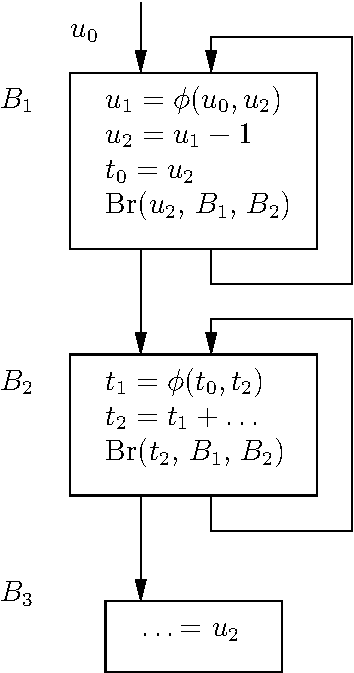
\includegraphics[width=0.7\textwidth]{cexple-impossible-1.fig}
  \end{minipage}
}
\hfill
\subfloat[ Branch with decrement (Br\_dec)]{
  \begin{minipage}{0.33\textwidth}
    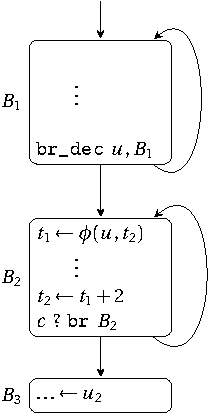
\includegraphics[width=0.7\textwidth]{cexple-impossible-2.fig}
  \end{minipage}
}
\hfill
\subfloat[CSSA with additional edge splitting]{
  \begin{minipage}{0.33\textwidth}
    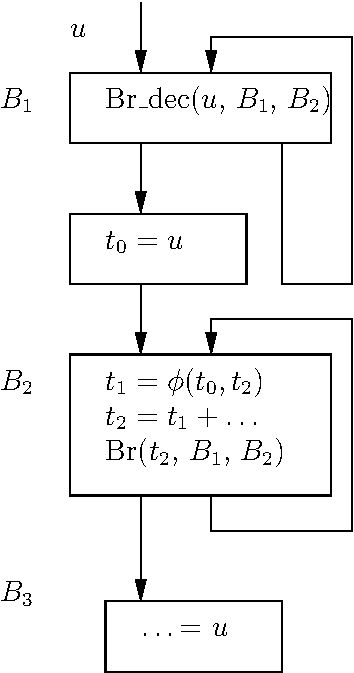
\includegraphics[width=0.7\textwidth]{cexple-impossible-3.fig}
  \end{minipage}
}
\caption{Copy insertion may not be sufficient.\label{fig:alternative_ssa_destruction:ex_jump_impossible}}
\end{figure}

{\bf Limitations}
There is a  tricky case, when the basic block contains variables
\emph{defined after} the point of copy insertion. This is the case for some
DSP-like branch instructions with a behavior similar to hardware looping. In
addition to the condition, a counter $u$ is decremented by the instruction
itself. If $u$ is used in a $\phi$-function in a direct successor block, no
copy insertion can split its live range. It must then be given the same name as
the variable defined by the $\phi$-function. If both variables interfere, this
is just impossible! To solve the problem, the SSA optimization could be
designed with more care, or the counter variable must not be promoted to SSA,
or some instruction must be changed, or the control-flow edge must be split
somehow.  SSA destruction by
copy insertion alone is not always possible, depending on the branch
instructions and the particular case of interferences.

For example, suppose that for the code of
Figure~\ref{fig:alternative_ssa_destruction:ex_jump_impossible}(a), the instruction selection chooses a branch
with decrement (denoted Br\_dec) for Block~$B_1$
(Figure~\ref{fig:alternative_ssa_destruction:ex_jump_impossible}(b)).  Then, the $\phi$-function of
Block~$B_2$, which uses $u$, cannot be translated out of SSA by standard copy
insertion because $u$ interferes with $t_1$ and its live range cannot be split.
To go out of SSA, one could add $t_1=u-1$ in Block~$B_1$ to anticipate the
branch. Or one could split the critical edge between $B_1$ and~$B_2$ as in
Figure~\ref{fig:alternative_ssa_destruction:ex_jump_impossible}(c). In other words, simple copy insertions is not enough in this case.


There is another tricky case when a basic-block have twice the same predecessor block. This can result from consecutively copy-folding and control flow graph structural optimizations like dead code elimination or empty block elimination. This is the case for the example of Figure~\ref{fig:alternative_ssa_destruction:doublepreds} where copy-folding\index{copy-folding} would remove the copy $a_2=b$ in basic-block $L_2$. If $L_2$ is eliminated, there is no way to implement the control dependence of the value to be assigned to $a_3$ other than through predicated code (see chapters~\ref{chapter:psi_ssa} and~\ref{chapter:vsdg}) or through the re-insertion of a basic-block between $L_1$ and $L_0$ by the split of one of the edges.

\begin{figure}[H]
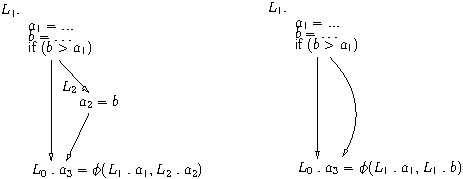
\includegraphics[width=0.5\textwidth]{doublepreds.fig}
\caption{\label{fig:alternative_ssa_destruction:doublepreds} Copy-folding followed by empty block elimination can lead to SSA code for which destruction is not possible through simple copy insertion}
\end{figure}

The last difficulty SSA destruction can face when performed at machine level is related to register constraints such as instruction set architecture (ISA)\index{instruction set architecture} or application binary interface (ABI)\index{application binary interface} constraints. For the sake of the discussion we differentiate two kinds of resource constraints that we will refer as \emph{operand pining}\index{pining} and \emph{live-range pining}. Live-range pining expresses the fact that the \emph{entire} live-range of a variable must reside in a given resource (usually a dedicated register). An example of live-range pining are versions of the stack-pointer temporary that must be assigned back to register \SP. On the other hand the pining of an operation's operand to a given resource does not impose anything on the live-range of the corresponding variable. The scope of the constraint is restricted to the operation. Examples of operand pining are operand constraints such as \emph{2-address-mode} where two operands of the same instruction must use the same resource; or where an operand must use a given register. This last case encapsulates ABI constraints. 
Note that more loose constraints where the live-range or the operand can reside in more than one resource are not handled here. We assume this to always be the responsibility of register allocation.

The live-range pining of a variable $v$ to resource $R$ will be represented $R_v$, just as if $v$ were a version of temporary $R$. An operand pining to a resource $R$ will be represented using the exponent $\pining{R}$ on the corresponding operand. 

We first simplify the problem by transforming any operand pining to a live-range pining as sketched in Figure~\ref{fig:alternative_ssa_destruction:pining}: parallel copies with new variables pined to the corresponding resource are inserted just before (for \useop pining) and just after (for \defop pining) the operation.

\begin{figure}[h]
\subfloat[Operand pining of an auto-increment]{
  \begin{minipage}{0.4\textwidth}
    $p_2\pining{T}=p_1\pining{T}+1$\\
  \end{minipage}
}
\hfill
\subfloat[Corresponding live-range pining]{
  \begin{minipage}{0.4\textwidth}
    $T_{p_2}=p_1$\\
    $p_2=T_{p_2}+1$
  \end{minipage}
}
\\
\subfloat[Operand pining of a function call]{
  \begin{minipage}{0.4\textwidth}
    $a\pining{R_0}=f(b\pining{R_0}, c\pining{R_1})$
  \end{minipage}
}
\hfill
\subfloat[Corresponding live-range pining]{
  \begin{minipage}{0.4\textwidth}
    $b'_{R_0}=b\ \parallel\ c'_{R_1}=c$\\
    $a'_{R_0}=f(b'_{R_0},c'_{R_1})$\\
    $a=a'_{R_0}$
  \end{minipage}
}
\caption{\label{fig:alternative_ssa_destruction:pining}Operand pining and corresponding live-range pining}
\end{figure}


{\bf Detection of strong interferences}
The scheme we propose in this section to perform SSA destruction that deals with machine level constraints does not address compilation cost (in terms of speed and memory footprint). It is designed to be simple. It first inserts parallel copies to isolate \phifuns and operand pining. Then it checks for interferences that would persist. We will denote such interferences as strong, as they cannot be tackled through the simple insertion of temporary-to-temporary copies in the code. We consider that fixing strong interferences should be done on a case by case basis and restrict the discussion here on their detection.

As far as correctness is concerned, Algorithm~\ref{alg:alternative_ssa_destruction:sreedhar} splits the data-flow between variables and \phinodes through the insertion of copies. For a given \phifun $a_0=\phi(a_1,\dots,a_n)$, this transformation is correct as soon as the copies can be inserted close enough to the \phifun. It might not be the case if the insertion point (for a \useop) of copy $a'_i\gets a_i$ is not dominated by the definition point of $a_i$; symmetrically, it will not be correct if the insertion point (for the \defop) of copy $a_0\gets a'_0$ does not dominate all the uses of $a_0$. Precisely this leads to inserting in Algorithm~\ref{alg:alternative_ssa_destruction:sreedhar} the following tests:
\begin{itemize}
\item line~\ref{line:sreedhar:1}: ``{\bf if} the definition of $a_i$ does not dominate $PC_i$ {\bf then} continue;''
\item line~\ref{line:sreedhar:2}: ``{\bf if} one use of $a_0$ is not dominated by $PC_0$ {\bf then} continue;''
\end{itemize}
We suppose a similar process have been performed for operand pining to express them in terms of live-range pining with very short (when possible) live-ranges around the concerned operations. 

At this point, the code is still under SSA and the goal of the next step is to check that it is conventional: this will obviously be the case only if all the variables of a \phiweb can be coalesced together. But not only: the set of all variables pined to a common resource must also be interference free. 
We say that $x$ and $y$ are \emph{pine-$\phi$-related} to one another if they are $\phi$-related or if they are pined to a common resource. The transitive closure of this relation defines an equivalence relation that 
partitions the variables defined locally in the procedure into equivalence classes, the pine-$\phi$-webs.
Intuitively, the pine-$\phi$-equivalence class of a resource represents a set of resources ``connected'' via \phifuns and resources.
The computation of \phiwebs given by Algorithm~\ref{alg:ssadestruction:find-webs} can be generalized easily to compute pined-\phiwebs. The resulting pseudo-code is given by Algorithm~\ref{alg:alternative_destruction_algorithm:web}. 

Now, one need to check that each web is interference free. A web contains variables and resources. The notion of interferences between two variables is the one discussed in Section~\ref{sec:properties_and_flavors:ultimate_interference} for which we will propose an efficient implementation later in this chapter. A variable and a resource do not interfere while two distinct physical resources will interfere with one another.

If any interference have been discovered, it has to be fixed on a case by case basis. Note that some interferences such as the one depicted in Figure~\ref{fig:alternative_ssa_destruction:doublepreds} can be detected and handled initially (through edge splitting if possible) during the copy insertion phase.


\begin{algorithm}
%% proc find_webs
%% // find the ssa web of each variable
\Begin{
\For{each resource $R$}{
  $\mathrm{web}(R)\gets \{R\}$\;
}
\For{each variable $v$}{
  $\mathrm{web}(v) \leftarrow \{v\}$\;
  \If{$v$ pined to a resource $R$}{
    union$(\mathrm{web}(R),\mathrm{web}(v))$
 }
}
\For{each instruction of the form $a_{\mathrm{dest}} = \phi(a_1,\ldots,a_n)$}{
  \For{each source operand $a_i$ in instruction}{
     union$(\mathrm{web}(a_{\mathrm{dest}}),\mathrm{web}(a_i))$
  }
}
}
\caption{\label{alg:alternative_ssadestruction_algorithm:find-webs}The pine-\phiwebs discovery algorithm, based on the union-find pattern}
\end{algorithm}

\section{Code Quality}
\section{Speed and Memory Footprint}
\section{Further Readings}

\section{Notes (to be removed)}

Define our ``ultimate'' notion of interference using value. Build the interference graph (provide the simplified pseudo-code). Do coalescing. Refer to CGO'09 paper for issues concerning JIT compilation. Remove \phifuns and perform renaming. Provide a more sophisticated pseudo-code (than for \ref{sec:classical_destruction}) for parallel copies sequentialisation (that can be performed before or after coalescing and $\phi$ removal.

Even this extremely conservative SSA destruction algorithm
can potentially lead to potential bugs,
particularly at the code generation stage.


%% +Pour l'implémenter on différentie resources et valeurs . La copie a->b%% +signifie que la valeur dans la resource a doit être copiee dans la
%% +resource b.  On racourcit en disant que la valeur ``a'' initialement
%% +dans la resource ``a'' doit être copiee dans la resource
%% +``b''.\\ Ainsi on maintient pour chaque valeur (v) dans quelle
%% +resource elle est disponible (Rcur(v)) et pour chaque resource (r)
%% +quelle valeur (s'il y en a une) elle devra contenir à la fin (Vend(r))
%% +(predecesseur dans le graphe).\\ On construit initialement et
%% +maintient la liste des feuilles ``leaves'' ie de resources qui ne
%% +contiennent pas de valeur (où bien la valeur est disponible
%% +ailleur). On est pour cela obligé de parcourir la liste des valeurs et
%% +marquer les resource qui contiennent une valeur. \\ On construit une
%% +autre liste ``todo'' qui est la liste des resources qui doivent avoir
%% +une valeur à la fin et qui ne contiennent pas cette valeur.\\ Si
%% +leaves n'est pas vide on pull une feuille b, et donc une copie de a->b
%% +avec a=Rcur(Vend(b)). On génère cette copie, et on set
%% +Rcur(Vend(b)):=b (la valeur Vend(b) qui était dans a est maintenant
%% +dans b). a est donc libérée de la valeur Vend et on push  a dans
%% +leaves.\\ Si leaves est vide, c'est soit que c'est terminé, soit qu'il
%% +y a un cycle sans duplication. Dans ce cas, on pull une resource a. Si
%% +Rcur(Vend(a))==a, a a déjà été traité, on passe. Sinon, on est en
%% +présence d'un cycl avec Rcur(a)=a. on génère une nouvelle variable
%% +(resource) a', on genère la copie a->a'. On met à jour Rcur(a):=a'. A
%% +est libéré, on le met dans leaves.
 
\begin{figure}[H]
\begin{minipage}{\textwidth}
\begin{minipage}[b]{0.23\textwidth}
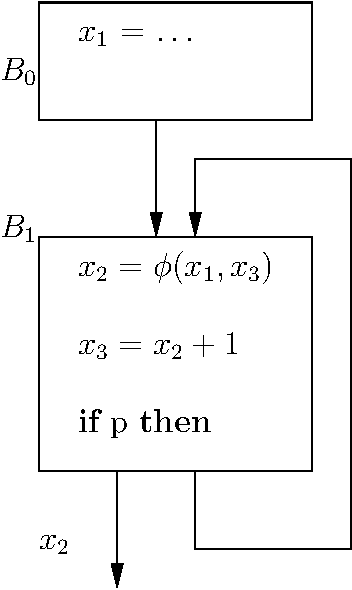
\includegraphics[width=0.7\textwidth]{lost.fig}

\centerline{a) Lost-copy problem}
\end{minipage}
\hfill
\begin{minipage}[b]{0.23\textwidth}
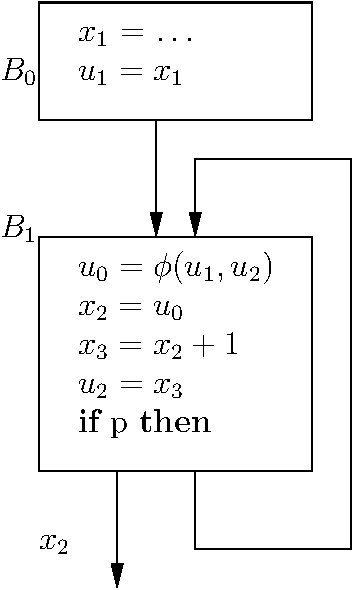
\includegraphics[width=0.7\textwidth]{lost2.fig}

\centerline{b) Corresponding CSSA code}
\end{minipage}
\hfill
\begin{minipage}[b]{0.23\textwidth}
\centerline{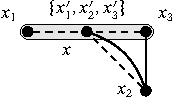
\includegraphics[width=0.7\textwidth]{lost-graph.fig}}

\centerline{c) Interferences and coalescing}
\end{minipage}
\hfill
\begin{minipage}[b]{0.23\textwidth}
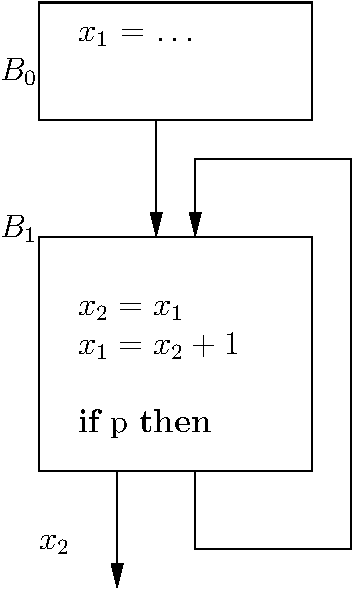
\includegraphics[width=0.7\textwidth]{lost3.fig}

\centerline{d) After copy optimization}
\end{minipage}
\end{minipage}
\caption{Out-of-SSA translation for the lost-copy problem.\label{fig:alternative_ssa_destruction:ex_lost}}
\end{figure}
